\documentclass[11pt,twoside]{scrartcl}
%\documentclass[11pt,twoside]{article}

%opening
\newcommand{\lecid}{15-316}
\newcommand{\leccourse}{Software Foundations of Security and Privacy}
\newcommand{\lecdate}{} %e.g. {October 21, 2013}
\newcommand{\lecnum}{14}
\newcommand{\lectitle}{Relaxing Noninterference}
\newcommand{\lecturer}{Matt Fredrikson}
\newcommand{\lecurl}{https://15316-cmu.github.io/index}

\usepackage{varwidth}
\usepackage{lecnotes}
\usepackage[irlabel]{bugcatch}

\usepackage{tikz}
\usetikzlibrary{automata,shapes,positioning,matrix,shapes.callouts,decorations.text,patterns,decorations.pathreplacing}

% \usepackage[bracketinterpret,seqinfers,sidenotecalculus]{logic}
% \newcommand{\I}{\interpretation[const=I]}

% \newcommand{\bebecomes}{\mathrel{::=}}
% \newcommand{\alternative}{~|~}
% \newcommand{\asfml}{F}
% \newcommand{\bsfml}{G}
% \newcommand{\cusfml}{C}
% \def\sqsubseteqftrule{L}%
% \def\rightrule{R}%

\begin{document}

\newcommand{\atrace}{\omega}%
%% the standard interpretation naming conventions
\newcommand{\stdI}{\dTLint[state=\omega]}%
\newcommand{\Ip}{\dTLint[trace=\atrace]}%
\newcommand{\ws}{\omega}\newcommand{\wt}{\nu}% 

\maketitle
\thispagestyle{empty}

%%%%%%%%%%%%%%%%%%%%%%%%%%%%%%%%%%%%%%%%%%%%%%

\section{Introduction}

In the previous two lectures, we have developed and studied a type system that enforces \emph{non-interference} (Definition~\ref{def:nonint}). Non-interference is a powerful information flow property, stipulating that variables assigned to designated ``high security'' classes have no influence over the values held in variables of lower-security classes. It is useful for establishing a number of security goals, such as \emph{confidentiality} and \emph{integrity}. 

The former goal concerns the flow of secret information out of a program through channels that may be observable to untrusted entities, and is perhaps the most commonly-cited use of non-interference in security. The latter goal, integrity, concerns the flow of untrusted information into a program, and is a key property to establish when one wants to eliminate the possibility of untrusted entities influencing critical parts of the program.

\begin{definition}[Non-interference]
\label{def:nonint}
Let $\asprg$ be a program and $\Gamma$ a type environment associating security labels to all of the variables in $\asprg$. Then $\asprg$ satisfies non-interference under $\Gamma$ if and only if executing $\asprg$ under \lowsec-equivalent states leads to final states that are also \lowsec-equivalent. More precisely,
\begin{equation}
\label{eq:noninterference}
\forall \omega_1,\omega_2 . \omega_1 \approx_{\Gamma,\lowsec} \omega_2 \land 
\langle \omega_1, \asprg\rangle \bigstep \omega_1' \land 
\langle \omega_2, \asprg\rangle \bigstep \omega_2'
\limply
\omega_1' \approx_{\Gamma,\lowsec} \omega_2'
\end{equation}
where $\omega_1$ and $\omega_2$ range over the set of possible program states.
\end{definition}

However, the stricture of non-interference can be problematic for many applications. Consider a program that authenticates users using passwords, using a database of credentials stored in local memory. It seems natural to apply non-interference to such a program to ensure that the secret credentials don't inadvertently leak out through public channels. A quick analysis of this proposal however indicates that it is doomed to failure, because of the necessary implicit flow that informs users of whether the password they provided is correct.

Our intuition tells us that there should be a way to formalize the security properties of such programs, as they have been used for decades without serious issue\footnote{There are indeed good arguments against using passwords for user authentication, but they mostly rest on the fact that everyday users tend to select poor passwords that are easy to guess. This is separate and orthogonal to the information flow security of password authentication programs.}. In today's lecture, we will see one such approach for \emph{relaxing} non-interference to allow for selected flows that have been deemed in advance to pose an insignificant threat to security.

\section{Relaxing non-interference: a simple example}

Let us continue with the example of a password-checking program, but because the programming language we work with only handles integer types, we will view passwords as personal identification numbers (PINs). To make things concrete, we will for now confine our discussion to the following program fragment that checks a user-provided ``guess'' against the value stored in a variable holding the correct PIN.
\begin{equation}
\mathit{auth} := 0; \pifs{\mathit{guess} = \mathit{pin}}{\mathit{auth}:=1}
\end{equation}
This program uses the variable $\mathit{auth}$ to hold the result of the authentication check, and will be communicated to the user to inform them of whether they are granted access to the system. So $\mathit{auth}$ must be \lowsec-typed, as must $\mathit{guess}$ which we assume holds the value of a variable provided by the user. But $\mathit{pin}$ should be \hisec-typed, because we don't want the correct value leaking to users who haven't provided the correct PIN.
What happens if we try to type this in the environment $\Gamma = (\mathit{auth} : \lowsec, \mathit{guess} : \lowsec, \mathit{pin} : \hisec)$? Obviously we can't do it, because the assignment to $\mathtt{auth}$ in the \hisec-typed scope will leak some information about \texttt{pw}. 

Why can't we just type $\mathit{auth}$ as \hisec? The point of an authentication routine like the one above is to determine when a user is among the list allowed to access the system. We must expect that some un-authentic users will attempt access, and when they do, it is unavoidable that our routine will let such users know that they have failed to authenticate. Thus, the value of \texttt{auth} needs to be typed \lowsec, or we will have no way of communicating this result back over a safe channel.

To address this problem in the special context of such authorization checks, in 1999 Dennis Volpano and Geoff Smith introduced a \keywordfont{match} expression into the information flow type system we've studied in this class~\cite{Volpano2000}. They introduced a corresponding typing rule that allows the result of a \keywordfont{match} expression to flow to the class corresponding to the least of its given operands.
\[
\cinferenceRule[match|Match]{Declassify Match}
{\linferenceRule[sequent]
  {
    \lsequent{\Gamma}{\astrm : \ell_1}
    &\lsequent{\Gamma}{\bstrm : \ell_2}
  }
  {\lsequent{\Gamma}{\pmatch{\astrm}{\bstrm} : \ell_1 \sqcap \ell_2}}
}{}%
\]
Where $\ell_1 \sqcap \ell_2$ denotes the \emph{greatest lower bound} of $\ell_1$ and $\ell_2$. Operationally, match just performs an equality test of its arguments. This makes it easy to rewrite our program from before.
\begin{equation}
\mathit{auth} := 0; \pifs{\pmatch{\mathit{guess}}{\mathit{pin}}}{\mathit{auth}:=1}
\end{equation}
Now we see that the assignment to \texttt{auth} will happen in a low context, because $\Gamma \vdash \keywordfont{match}(\mathtt{guess},\mathtt{pw}) : \lowsec \sqcap \hisec$, and $\lowsec \sqcap \hisec = \lowsec$.

\paragraph{Understanding leakage.} Is this a good idea? The programs that our new type system with \irref{match} verifies no longer need to satisfy noninterference. Now the question of whether a well-typed program protects secret information is more subtle, because we don't have the straightforward all-or-nothing definition of noninterference to rely on.

Although our intuition (and decades of experience) tells us that breaking noninterference in the way that many authorization checks do is probably fine, there may be other programs we could write in this new language that aren't so well-behaved. For example, we could write the following program:
\[
\mathit{guess := 0; \pwhile{\lnot\pmatch{\mathit{guess}}{\mathit{pin}}}{\mathit{guess}:=\mathit{guess}+1}}
\]
If an attacker with unsavory goals can manage to run this program on the system holding $\mathtt{pin}$, then the final value of $\mathtt{guess}$ will leak the \emph{entire} contents of $\mathtt{pin}$!

We know that adding \keywordfont{match} to our language makes it \emph{possible} for a program to leak the contents of an \hisec-typed variable into an \lowsec variable, \emph{but perhaps this does not imply that doing so is feasible}. In this case, the attacker may need to let the program run for time $O(2^k)$, assuming $\mathtt{pin}$ is a $k$-bit secret. Intuitively it seems that this complexity is the best an attacker can do given \keywordfont{match}, but can we formalize this intuition to get a guarantee that bounds the attacker's complexity when attempting such a leak?

Essentially, we want to state a guarantee that any attacker who uses \keywordfont{match} to learn the secret value requires time exponential in the size of the secret. But there are a few subtleties we should think about when postulating this guarantee.
\begin{description}
\item[\ \ Deterministic vs. non-deterministic attackers.] Although we've only talked about deterministic semantics for our language, it's good to be explicit about limitations when stating a formal guarantee. In particular, if we were to extend the language with non-deterministic commands, then keeping our relaxed rule for \keywordfont{match} would be a bad idea. The attacker could then non-deterministically choose a value for \texttt{guess}, compute the value of $\keywordfont{match}(\mathit{guess},\mathit{pin})$, and if it returns $\keywordfont{true}$, learn the secret in constant time.

\item[\ \ Distribution of secrets.] You may already be familiar with the fact that users tend to pick bad passwords that are far easier to guess than a naive bound based on plain bit-length would suggest. Formally, we characterize this fact in terms of the probability distribution corresponding to passwords selected by users in the ``real world''. The fact that this distribution is not uniform, i.e., does not assign equal probability to all possible passwords, is what makes password-guessing easier than $O(2^k)$ in practice. 

Formalizing real-world distributions is hard. To make our guarantee generalize to any type of secret, we won't make any assumptions about the distribution of values for the secret, so our formal statement will need to be \emph{qualitative} and \emph{universal}. In other words, we'll characterize the complexity of an attacker who attempts to copy a secret from \emph{any} distribution (i.e., universal), and we'll only worry about whether this attacker can succeed all the time or some of the time (i.e., qualitative).

\item[\ \ Secret size.] We assume that the secret value is stored in the memory of a real machine, so it must have a finite length of $k$ bits, for some $k$. For any fixed $k$, there exists a polynomial-time attacker who can brute-force the secret using the program above. So our guarantee will need to refer to an attacker who attempts to learn a secret of \emph{any} size in polynomial time.
\end{description}

Putting this all together, we can state our guarantee as the following theorem, due to Volpano and Smith~\cite{Volpano2000}.

\begin{theorem}
\label{thm:match}
Let $\Gamma = (s : \hisec, o : \lowsec)$ and $\asprg$ be a deterministic program such that:
\begin{enumerate}
\item $\lsequent{\Gamma}{\asprg}$ in the type system that includes $\keywordfont{match}$. 
\item $\langle \omega, \asprg\rangle \Downarrow \nu$ for $\omega(s) = v, \omega(o) \ne v, \nu(o) = v$.
\end{enumerate}
In other words, $\asprg$ always succeeds at transferring the value stored in $s$ at the initial state into $o$ at the final state. Then there exists some state $\hat{\omega}$ where:
\begin{enumerate}
\item $\hat{\omega}(s)$ requires at least $k$ bits to represent
\item Evaluating $\langle\hat{\omega},\asprg\rangle$ results in greater than $\mathit{poly}(k)$ evaluations of \keywordfont{match}.
\end{enumerate}
In other words, the type system prevents polynomial-time attacks on some \hisec state.
\end{theorem}

\begin{proof}
We'll begin with the intuition behind the proof. The only way for the value of $\mathtt{s}$ to influence the value of $\mathtt{o}$ is via calls to $\keywordfont{match}$, and each call either eliminates one possible value of $\mathtt{s}$ from the adversary's list of candidates to consider, or confirms the correct value. A $k$-bit variable encodes $2^k$ possible values, so we just need to choose $k$ large enough that $\asprg$ can't make enough calls to $\keywordfont{match}$ to distinguish between all the possible values.

Suppose that $\asprg$ runs in time $\mathit{poly}(k)$. Choose $k$ large enough such that $2^k > \mathit{poly}(k)+1$. Note that $\asprg$ can only call $\keywordfont{match}$ at most $\mathit{poly}(k)$ times, so there must be a pair of $k$-bit values $x \ne y$ such that $\asprg$ doesn't evaluate $\keywordfont{match}(o,s)$ in either state $\omega(o) = x, \omega(o) = y$. Then because $\asprg$ is deterministic, if $\asprg$ is to end in $\nu(o) = x$ when started in $\nu(s) = x$, it must also end in $\nu(o) = x$ when started in $\nu(s) = y$. Thus the assumption that $\asprg$ runs in $\mathit{poly}(k)$ is in conflict with the assumptions made of $\asprg$ in the theorem statement.
\end{proof}

\textbf{Question.} \emph{Theorem~\ref{thm:match} makes a fairly specific, and one might argue narrow, statement about the complexity of attacking a secret using \keywordfont{match}. Are you convinced by this result? Could you make the result stronger without changing the operational semantics of \keywordfont{match}? How might you make small changes to \keywordfont{match} to allow for a stronger statement? Are there assumptions that one might make about an implementation of \keywordfont{match} (ideally ones that can be realized in practice) to strengthen the result?}

\section{Declassification: A Taxonomy}

The \irref{match} rule is a simple example of a \emph{declassification} mechanism. In general, we can think of a richer space of mechanisms for making information flow protection less rigid than noninterference. One useful way of characterizing declassification mechanisms places them along several dimensions~\cite{Sabelfeld09}: \emph{what} information is released, \emph{where} controls the release, \emph{who} is allowed to see it, and \emph{when} the release occurs.

\begin{description}
\item[\ \ What.] The \keywordfont{match} construct only allows us to declassify one particular type of information: the result of an equality comparison between a (potentially) \hisec and \lowsec variable. This is a type of \emph{partial} information about the \hisec variable, but we could imagine other forms of partial information we may want to release, such as other comparisons, aggregates, and samples.

\item[\ \ Where.] We might also imagine releasing information without sacrificing control over where it could eventually end up. The type system we have already discussed employs a security lattice to do this in one way; a partial order on lattice elements denotes how information is allowed to flow between variables (i.e., $\ell_1 \sqsubseteq \ell_2$ means that information in an $\ell_1$ variable can flow to one typed $\ell_2$, but not the other way around). Apart from controlling ``where'' in terms of levels, we can also think of doing so in terms of code location. By defining which parts of the code are allowed to read certain pieces of information, we can ensure that potentially untrusted parts aren't able to leak them any further.

\item[\ \ Who.] The information flow type system we've discussed doesn't explicitly differentiate between principals, but one could design a system that tracks who owns a particular piece of information. With this information, it would then be possible to specify that certain types of declassification are allowed when the owner of the data requests them, but not on behalf of any other users. These systems can be further extended with delegation for additional flexibility. However, one must be careful to ensure that such mechanisms can't be abused by attackers.

\item[\ \ When.] Time can play a nuanced role in declassification. In the example we discussed at the beginning of lecture, we essentially relied on an argument about timing to justify the safety of \keywordfont{match}. Namely, because the secret won't be leaked in polynomial time, we decided it was safe to release partial information. Another nuanced application of timing in declassification mechanisms might crop up in the form of a probabilistic guarantee, which states that a secret will only be released with some small probability. Essentially, this is an argument that secrets will be leaked infrequently (assuming the distribution used aligns well enough with realistic assumptions). Finally, timing can play a more obvious role, such as with policies that dictate the release of information relative to the occurrence of other events on the system. For example, a digital media retailer might use a policy which states that the DRM key for a particular title can be released to the user once payment has been confirmed.
\end{description}

We won't explore every dimension of this taxonomy in greater detail today, and will instead focus primarily on the \textbf{what}. However, you should consider approaches that we've already discussed, in addition to those we'll discuss later on, in the context of this taxonomy. Doing so will highlight the primary differences between different approaches to information protection and what they are trying to achieve, which can be helpful when trying to distinguish important high-level (and perhaps generally-applicable) ideas from incidental low-level details.

\section{Formalizing Leakage}

\paragraph{Attacker model.}
The notion of observability is central to precisely defining an information flow attacker. We assume that the adversary is able to observe and influence certain aspects of the program and its execution, and we're interested in understanding exactly what the attacker can deduce about the secret parts of the initial program state.

\begin{itemize}
\item As we did before when we formalized noninterference, we'll define a security lattice $L = (SC, \sqsubseteq, \sqcup, \sqcap, \perp)$. To keep things simple, we'll use the two-point lattice $SC = \{\lowsec, \hisec\}$ where $\lowsec = \perp \ne \hisec$, so $\lowsec \sqsubseteq \hisec$ and $\hisec \not\sqsubseteq \lowsec$.

\item We assume that the attacker knows the code of the program that is executing. It may seem that this gives our attacker quite a bit of power that may be unrealistic in some cases, but it frees us from needing to consider whether the attacker is able to learn this information using other means.

\item We assume that there are two moments in time at which the attacker can make observations about the program state: before the program is run (i.e., the initial state $\omega$), and after it finishes executing (i.e., the final state $\omega'$). We won't worry about nonterminating programs for the time being, although termination behavior could be relevant to information flow.

\item We associate the attacker with the lattice element $\lowsec$, and assume that the attacker can observe any \lowsec-typed variable in $\omega$ and $\omega'$. We'll write $\omega_L$ and $\omega'_L$ to denote the portions of the initial and final states, respectively, that correspond only to the \lowsec variables.

\item We provision our attacker with the ability to make arbitrary assignments to the \lowsec-typed variables in the initial state $\omega$.

\item Finally, we place no immediate constraints on the time or space complexity of the attacker. In certain situations we may attempt to characterize how powerful an attacker needs to be, in terms of time and space resources, but unless otherwise stated, we assume that the attacker has unlimited resources.
\end{itemize}

To summarize, our attacker has total knowledge of the program being executed, along with the ability to decide which values \lowsec-typed variables take in the initial state, and to observe the values of \lowsec-typed variables in the initial and final states. The attacker's goal is to determine which values the \hisec-typed variables take in the initial state.

\paragraph{Feasible sets and indistinguishability.} We've introduced the big-step operational semantics previously, characterizing it in terms of the following relations for expression and programs, respectively:
\[
\langle \omega, \astrm\rangle \Downarrow v
\quad\quad\quad\quad\quad\quad\quad\quad
\langle \omega, \asprg\rangle \Downarrow \omega'
\]
Given a state $\omega$ mapping variables to values and expression $\astrm$ (resp. program $\asprg$), evaluation results in a value $v$ (resp. state $\omega'$). When relating the results of different evaluations, it becomes unwieldly to use this notation, as it requires introducing new ``temporary'' variables to hold the result of each evaluation.

We'll simplify matters a bit by introducing a new notation:
\[
\eval{\omega}{\astrm}
\quad\quad\quad\quad\quad\quad\quad\quad
\eval{\omega}{\asprg}
\]
$\eval{\omega}{\astrm}$ (resp. $\eval{\omega}{\asprg}$) refers to the value (resp. state) obtained by evaluating $\astrm$ (resp. $\asprg$) in $\omega$.

The only way in which our attacker has to go about learning the \hisec-typed values is by comparing their observations of the \lowsec-typed parts of the initial and final states, $\omega$ and $\eval{\omega}{\asprg}$ with their knowledge of the program's semantics, and deducing which values of the initial \hisec variables are \textbf{feasible}, or consistent with her observations and the program semantics. Note that because programs are deterministic, once the intiial \hisec values are known, the attacker can deduce them for any other point in the program's execution.

We formalize this idea by defining the \textbf{feasible set} given a program $\asprg$, context $\Gamma$, and initial state $\omega$, using the notation $\Omega_{\Gamma}(\asprg,\omega)$ for shorthand. This is nothing more than the set of initial states that \emph{agree with the attacker's knowledge of the \lowsec values of the initial and final states}:
\[
\Omega_\Gamma(\asprg,\omega) =
\{
 \omega' \with \omega' \approx_\lowsec \omega~\text{and}~\eval{\omega'}{\asprg} \approx_\lowsec \eval{\omega}{\asprg}
\}
\]
The feasible set characterizes all of the attacker's knowledge of what the initial state, and in particular the \hisec part of the initial state (because the rest is known), could be given the available information. Intuitively, any state in the feasible set will lead to \emph{exactly} the same observations in the initial and final states, and so the attacker has no way of determining which of these states the program actually started in. From the attacker's perspective, they are \emph{indistinguishable} from each other.

\begin{example}
Let's go back to the \keywordfont{match} construct from earlier, and work out the feasible set. Suppose that we have a very simple program that consists of a single evaluation of \keywordfont{match}.
\begin{equation}
o := \pmatch{l}{h}
\end{equation}
We'll assume that $\Gamma = (o : \lowsec, l : \lowsec, h : \hisec)$, so the attacker can set the value of $l$ to whatever they likes in the initial environment, and observe the value of $o$ afterwards. The goal, of course, is to learn the value $h$ holds in the initial state.

Suppose that we, playing the role of an attacker, choose to run the program in an environment where $\omega(l) = v$, and in the final environment $\nu$ observe that $\nu(o) = 0$. While this does not allow us to deduce the exact value of $\omega(h)$, we haven't come away completely empty-handed, because we know that $\omega(h) \ne v$. We can deduce this by reasoning counterfactually, supposing what \emph{would have} happened in either situation:
\begin{itemize}
\item In the case where $\omega(h) = v$, reasoning by our knowledge of the program and the operational semantics tells us that:
\[
\langle \omega, \keywordfont{match}(l, h) \rangle \Downarrow \nu~\text{where}~\nu(o)=1
\]
In other words, if $\omega(h) = v$ in the initial state, then we would expect to see $\nu(o) = 1$ in the final state.

\item In the case where $\omega(h) = v'$, where $v' \ne v$, reasoning by our knowledge of the program tells us that:
\[
\langle \omega, \keywordfont{match}(l,h) \rangle \Downarrow \nu~\text{where}~\nu(o)=0
\]
This is exactly what we observed when we ran the program, so we conclude that $\omega(h) \ne v$.
\end{itemize}
So although we didn't learn the whole value of $\omega(\mathtt{h})$, we were able to rule exactly one potential value out as impossible given our observations. In this case, after running the program a single time in an initial state where $\omega(l) = v$, we end up with the feasible set:
\[
\Omega_\Gamma(\asprg,\omega) = 
\{
\omega' \with \omega'(h) \ne v
\}
\]
On the other hand, by our reasoning above, if we had observed $\omega'(\mathtt{o}) = 1$, then we would have had:
\[
\Omega_\Gamma(\asprg,\omega) = 
\{
\omega' \with \omega'(h) = v
\}
\]
The feasible sets and their corresponding deductions are depicted in the diagram below.
\begin{center}
\resizebox{0.45\textwidth}{!}{%
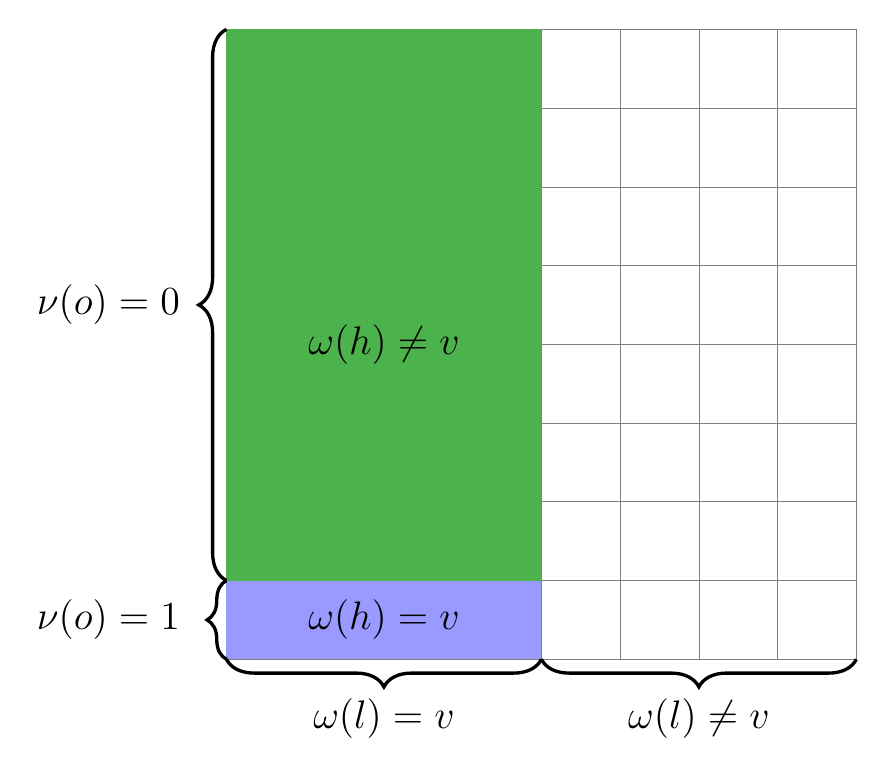
\begin{tikzpicture}
\draw[step=1cm,gray,very thin] (-2,-2) grid (6,6);
\fill[blue!40!white] (-2,-2) rectangle (2,-1);
\fill[green!40!gray] (-2,-1) rectangle (1,6);
\fill[green!40!gray] (1,-1) rectangle (2,1);
\fill[green!40!gray] (1,1) rectangle (2,6);

\node at (0,-1.5) {\Large $\omega(h) = v$};
\node at (0,2) {\Large $\omega(h) \ne v$};

\draw [very thick,decorate,decoration={brace,amplitude=10pt,mirror},yshift=0pt]
(-2,-2) -- (2,-2) node [black,midway,yshift=-0.75cm] 
{\Large $\omega(l) = v$};

\draw [very thick,decorate,decoration={brace,amplitude=10pt,mirror},yshift=0pt]
(2,-2) -- (6,-2) node [black,midway,yshift=-0.75cm] 
{\Large $\omega(l) \ne v$};

\draw [very thick,decorate,decoration={brace,amplitude=7pt},yshift=0pt]
(-2,-2) -- (-2,-1) node [black,midway,xshift=-1.5cm] 
{\Large $\nu(o) = 1$};

\draw [very thick,decorate,decoration={brace,amplitude=10pt},yshift=0pt]
(-2,-1) -- (-2,6) node [black,midway,xshift=-1.5cm] 
{\Large $\nu(o) = 0$};

\end{tikzpicture}
}
\end{center}
Each region of the diagram depicts a set of possible initial states, the notations on curly braces correspond to observations that the attacker can make, and the text inside each region corresponds to deductions that the attacker can make about \hisec-typed variables. Obviously, the attacker knows that $\omega(l) = v$, which allows elimination of the right half of the figure. After setting $\omega(l) = v$ in the initial state and observing $\nu(o) = 1$ in the final state, the attacker can conclude that $\omega(h) = v$, or $\omega(h) \ne v$ in the case where $\nu(o) = 0$.
\hfill\rule{2mm}{2mm}
\end{example}

\begin{example}
Recall the definition of noninterference from an earlier lecture:
\[
\forall \omega_1, \omega_2 . \omega_1 \approx_\lowsec \omega_2 \land \langle \omega_1, P \rangle \Downarrow \omega_1' \land \langle \omega_2, P \rangle \Downarrow \omega_2'\ \Longrightarrow\ \omega_1' \approx_\lowsec \omega_2'
\]
In the notation introduced today, we can simply write:
\[
\forall \omega_1, \omega_2 . \omega_1 \approx_\lowsec \omega_2\ \Longrightarrow\ \eval{\omega_1}{P} \approx_\lowsec \eval{\omega_2}{P}
\]
What is the feasible set for any program that satisfies noninterference?
Looking at the definition, notice the universal quantifier which says that \emph{all} \lowsec-equivalent initial states will lead to exactly the same final-state observation, so executing the program won't allow us to eliminate any more possible states from the feasible set than those not satisfying $\omega_I \approx_\lowsec \omega_\lowsec$. This leaves us with the set:
\[
\Omega_\Gamma(\asprg,\omega) = \{ \omega' \with \omega' \approx_\lowsec \omega \}
\]
which does not eliminate any possible values for \hisec variables, so no information is leaked.
\hfill\rule{2mm}{2mm}
\end{example}

Notice in the first example two very different feasible sets. In one case, where \keywordfont{match} returns 0, the attacker is left with many feasible values; in fact, only one value is eliminated, so there are $2^n-1$ elements assuming $n$ bits to represent the \hisec part of $\omega$. 

In the second case, there is exactly one feasible element that remains, so the attacker has complete knowledge of the \hisec state. The cardinality of the feasible set is one way of measuring the degree to which $P$ leaks information about \hisec state, quantitatively. Indeed, this is why we were able to prove the theorem from before: \keywordfont{match} does not give the attacker a reliable way of obtaining a small feasible set, so it is difficult to obtain much information about the \hisec initial state. 

\textbf{Question.} \emph{What would happen if instead of allowing \keywordfont{match}, we allowed an expression $\keywordfont{compare}(a_1,a_2)$ which returns 1 iff $a_1 < a_2$, to be given the type $\ell_1 \sqcap \ell_2$? Can the attacker reliably obtain feasible sets that are small enough to effeciently learn the secret?}

\section{Explicit Declassification}

Suppose that we extend our language with a more general-purpose declassification mechanism, by means of an expression called \keywordfont{declassify}. The expression \keywordfont{declassify} takes a single argument, which is another expression, and works as follows.
\begin{enumerate}
\item Operationally, \keywordfont{declassify} simply returns the value of its argument.
\item In the type system, \keywordfont{declassify} always types as the least element $\bot$, which in our running example two-label lattice is \lowsec, so it does not prevent leaking its value to any variable.
\end{enumerate}
The typing logic is formalized in the rule below.
\[
\cinferenceRule[declass|Declass]{Declassify Expression}
{\linferenceRule[sequent]
  {}
  {\lsequent{\Gamma}{\pdeclass{\astrm} : \bot}}
}{}%
\]
We could also consider generalizing even further, supporting a $\keywordfont{declassify}_\ell$ expression for each label $\ell$ in the lattice. The corresponding typing rule would be as shown below.
\[
\cinferenceRule[declassl|DeclassL]{Declassify Expression}
{\linferenceRule[sequent]
  {}
  {\lsequent{\Gamma}{\keywordfont{declassify}_\ell(\astrm) : \ell}}
}{}%
\]
To keep things simple, we'll stick with the former expression \keywordfont{declassify} for the rest of the lecture.
Notice that this mechansim generalizes the sort of functionality we obtained from \keywordfont{match}.
\[
\mathit{auth} := 0; \pifs{\pdeclass{\mathit{guess}=\mathit{pin}}}{\mathit{auth}:=1}
\]
But we can also do other useful things with it. For example, suppose we have a set of variables $s_1, \ldots, s_{100}$ containing the salaries of 100 employees. Before, if we wanted to extract any useful information from this data while still obtaining any degree of information security regarding its entire contents, there were few options. Noninterference wouldn't allow us to release an aggregate like the average, so our type system wouldn't allow the program to run. But if we wrap an expression computing the average in \keywordfont{declassify}, we are allowed to save the result to \lowsec variables.

However, this flexibility is sufficiently powerful that we can also do very bad things, like simply declassifying variable expressions containing secret data. Thus, when using \keywordfont{declassify}, it's important to understand what's being leaked. We can reason in terms of feasible sets and indistinguishability to figure this out.

\paragraph{Indistinguishability and declassification.}
The \keywordfont{declassify} construct gives us an ``escape hatch'' through which we can selectively relax the stricture of noninterference. Citing again the definition of noninterference, let's think about what \keywordfont{declassify} changes:
\[
\forall \omega_1, \omega_2 . \omega_1 \approx_\lowsec \omega_2 \Longrightarrow\ \eval{\omega_1}{P} \approx_\lowsec \eval{\omega_2}{P}
\]
Noninterference says that whenever our initial states are indistinguishable on \lowsec variables, then our final states will be too. In correspondence with this notion, we assume that an attacker can observe all the \lowsec variables in both states.

With \keywordfont{declassify}, we make a different assumption. Namely, by typing all \keywordfont{declassify} expressions as \lowsec, we assume that the attacker is able to observe the value of all such expressions. In other words, given two states $\omega_1, \omega_2$:
\begin{itemize} 
\item If their values differ in a way that can be observed through a \keywordfont{declassify} escape hatch, then we want to allow it.
\item However, \keywordfont{declassify} doesn't allow \emph{arbitrary} leaks. If there is a difference between the \hisec variables in $\omega_1,\omega_2$ that can't be detected through the value of \keywordfont{declassify}, i.e. does not result in different values of the expressions wrapped in \keywordfont{declassify}, then the attacker won't be able to distinguish them.
\end{itemize}
Armed with this intuition, we can formalize the indistinguishability guarantee that \keywordfont{declassify} gives us. Namely, we can \emph{weaken} noninterference by adding a condition to the antecedent of the implication. For a program with a single \keywordfont{declassify} wrapping an expression $\astrm$, perhaps we can say that:
\begin{equation}
\label{eq:declass-leakage}
\forall \omega_1, \omega_2 . \omega_1 \approx_\lowsec \omega_2 \land \eval{\omega_1}{e} = \eval{\omega_2}{e} \Longrightarrow\ \eval{\omega_1}{P} \approx_\lowsec \eval{\omega_2}{P}
\end{equation}
The property shown in Equation~\ref{eq:declass-leakage} is more subtle than it may seem. To see why, consider the following program.
\begin{equation}
\begin{array}{l}
s_2 := s_1; \\
s_3 := s_1; \\
\vdots \\
s_{100} := s_1 \\
o := \pdeclass{(s_1 + s_2 + \cdots + s_{100})/100}
\end{array}
\end{equation}
When this program terminates, $\mathit{avg}$ will contain exactly the initial value of $s_1$. However, given two initial states $\omega_1, \omega_2$ in which $\eval{\omega_1}{s_1 + \cdots + s_{100}} = \eval{\omega_2}{s_1 + \cdots + s_{100}}$, it will not be the case that $\eval{\omega_1}{\asprg} = \eval{\omega_2}{\asprg}$.

The problem is due to the fact that the \hisec variables appearing in the \keywordfont{declassify} expression were assigned before being used in the \keywordfont{declassify}, so that the declassified value differs from the indistinguishability condition in Theorem~\ref{thm:declass-security}. So to ensure that the leakage characterized in Equation~\ref{eq:declass-leakage} aligns with our intuition of what \keywordfont{declassify} means, we need to require that certain variables not change from their initial values prior to their use in a \keywordfont{declassify}. 

\begin{theorem}
\label{thm:declass-security}
Let $P$ be a deterministic program such that:
\begin{enumerate}
\item $\Gamma \vdash P$ in the type system that includes $\mathbf{declassify}$. 
\item $P$ contains exactly one instance of $\mathbf{declassify}(e)$, over expression $e$.
\item None of the variables mentioned in $e$ are assigned within the program before the $\mathbf{declassify}$ occurs.
\end{enumerate}
Then the following holds:
$
\forall \omega_1, \omega_2 . \omega_1 \approx_\lowsec \omega_2 \land \eval{\omega_1}{e} = \eval{\omega_2}{e} \Longrightarrow\ \eval{\omega_1}{P} \approx_\lowsec \eval{\omega_2}{P}
$.
In other words, whenever the initial states are indistinguishable under the declassification expression, then the resulting final states will be indistinguishable as well.
\end{theorem}

\begin{proof}
Proving this theorem is a good exercise that you should consider doing when preparing for the final exam. If you have trouble, ask the course staff for some hints or consult Sabelfeld and Myers~\cite{Sabelfeld04}.
\end{proof}

This theorem formalizes the intutition we developed above. The additional requirement imposed by (3) means that if we wanted to obtain the protection guaranteed by Theorem~\ref{thm:declass-security} using a type system, then we would need to design the rules so that \emph{only} instances of \keywordfont{declassify} whose constituent variables have never been assigned can be given the type \lowsec.

\bibliography{bibliography}
\end{document}